\documentclass[12pt,a4paper]{article}
\usepackage{ngerman}
\usepackage[utf8]{inputenc}
\usepackage{sectsty, xcolor}
\usepackage{lastpage}
\usepackage{amsfonts, amssymb, array, enumitem, fancyhdr, graphicx, float, makeidx, textcomp, multicol, tabularx}
\usepackage[fleqn]{amsmath} %Math-Environment linksbündig
\usepackage{MnSymbol}
\usepackage[hidelinks]{hyperref}
\usepackage[hang,flushmargin]{footmisc}
\usepackage{tikz}

\newcolumntype{Y}{>{\centering\arraybackslash}X}

\setlist[itemize]{noitemsep,topsep=0pt,leftmargin=*}
\setlist[enumerate]{noitemsep,topsep=0pt,leftmargin=*}
\setlength\parindent{0pt}

\makeindex

% \definecolor{dunkelblau}{rgb}{0,0.4,0.6}
% \subsectionfont{\color{dunkelblau}}

\title{ANLIS HS 2020}
\author{Victor Fernández}
\date{}

\addtolength{\oddsidemargin}{-.875in}
\addtolength{\evensidemargin}{-.875in}
\addtolength{\textwidth}{1.75in}
\addtolength{\topmargin}{-.875in}
\addtolength{\textheight}{1.75in}

% muss nach Änderung der margin kommen!
\pagestyle{fancy}
\fancyhf{} %reset
\fancyhead[L]{HSLU}
\fancyhead[C]{ANLIS}
\fancyhead[R]{\thepage/\pageref{LastPage}}
\fancyfoot[L]{}
\fancyfoot[C]{}
\fancyfoot[R]{}
\renewcommand{\headrulewidth}{0.2pt} % Strich in Kopfzeile

\newcommand{\todo}[1]{\textcolor{red}{//TODO: #1//\\[1em]}}

\begin{document}

\maketitle
\tableofcontents
\thispagestyle{empty}
\pagebreak
\part{SW 01 - Networking Today \& Networking Trends}
\section{Lernziele (Leitfragen)}
\begin{enumerate}
    \item Wieso sind Computernetzwerke wichtig in unserem Leben?
    \item Wieso sind Computernetzwerke wichtig für Unternehmen und unsere Berufe?
    \item Wieso ist Kenntnis der Computernetzwerke wichtig für die Wirtschaftsinformatik?
    \item Was ist ein \flqq End Device\frqq{} (Endgerät)? Geben Sie Beispiele.
    \item Was ist ein ``intermediary (network) device'' (Netzwerkkomponente), oder Netzwerkgerät? Geben Sie Beispiele.
    \item Wie funktioniert das \flqq Client-Server\frqq{} Modell? Geben Sie Beispiele.
    \item Wie funktioniert das \flqq Peer-to-peer\frqq{} Modell? Geben Sie Beispiele.
    \item Wie unterscheiden sich physikalische und logische Netzwerkdiagramme?
    \item Wie kann man anhand ihrer Grösse Computernetzwerke klassifizieren?
    \item Wie unterschieden sich LANs und WANs? Was ist ihre Beziehung?
    \item Was ist das Internet? Wer besitzt das Internet? Was für Organisationen sind in der Entwicklung des Internets beteiligt?
    \item Was ist der Unterschied zwischen einem Intranet und einem Extranet?
    \item Wie verbinden sich normalerweise Häuser, Wohnungen und HomeOffices mit dem Internet?
    \item Wie verbinden sich normalerweise Büros und Unternehmern mit dem Internet?
    \item Was bedeutet Konvergenz im Kontext der Computernetzwerke?
    \item Was bedeutet \flqq fault tolerance\frqq{}  (Fehlertoleranz) im Kontext der Computernetzwerke? Geben Sie ein Beispiel
    \item Was bedeutet \flqq scalability\frqq{}  (Skalierbarkeit) im Kontext der Computernetzwerke? Geben Sie ein Beispiel
    \item Was bedeutet \flqq quality of service (QoS)\frqq{}  im Kontext der Computernetzwerke? Geben Sie ein Beispiel
    \item Wieso ist Netzwerksicherheit wichtig?
    \item Was sind die drei Hauptinformationssicherheitsziele?
    \item Was ist \flqq BYOD\frqq{}  und was sind seine Auswirkungen für Geschäfte und Unternehmen?
    \item Was ist \flqq cloud computing\frqq{} ? Was für Cloud Arten gibt es?
    \item Was ist die Verbindung zwischen \flqq cloud computing\frqq{}  und Computernetzwerken?
\end{enumerate}

\section{Antworten}
\subsection*{Wieso sind Computernetzwerke wichtig in unserem Leben?}
Die zunehmende Digitalisierung erfordert eine immer grössere Vernetzung im Alltag. Sei es beruflich mit E-Mails, Website, Dateitransfer, cloudbasierte Lösungen etc. oder auch privat mit digitalem Fernsehen, Streamingangeboten von Videos und Musik, bis zur Smart-Watch.
\subsection*{Wieso sind Computernetzwerke wichtig für Unternehmen und unsere Berufe?}
Für moderne Unternehmen ist es heutzutage wichtig vernetzt zu sein. Man verfügt beispielsweise über IP-Telefone, Fileserver, Mailserver, Virtual-Machine-Server, Rendering-Server etc. Um auf all diese Dienste zugreifen zu können, muss ein Computernetzwerk bestehen.
\subsection*{Wieso ist Kenntnis der Computernetzwerke wichtig für die Wirtschaftsinformatik?}
Die Berufsausrichtung/-aussicht der Wirtschaftsinformatikspezialisten tendiert dazu, dass sie leitende Angestellte werden. Genehmigungen für Budgetanträge im Bereich der Informatik erfordern daher ein gutes Know-How von Komponenten, die in der Branche verwendet werden.
\pagebreak
\subsection*{Was ist ein \flqq End Device\frqq{} (Endgerät)? Geben Sie Beispiele.}
\begin{itemize}
    \item Smartphone \& IP-Telefone
    \item Drucker
    \item Notebook
    \item Server (physisch)
    \item Tablet
    \item IoT-Geräte\footnote{Internet of Things - vom intelligenten Kühlschrank bis zum selbstfahrenden Auto.}
\end{itemize}
\subsection*{Was ist ein ``intermediary (network) device'' (Netzwerkkomponente), oder Netzwerkgerät? Geben Sie Beispiele.}
\begin{itemize}
    \item (Wireless) Router
    \item LAN \& Multilayer Switches
\end{itemize}
\subsection*{Wie funktioniert das \flqq Client-Server\frqq{} Modell? Geben Sie Beispiele.}
Das Modell beschreibt die Rolle eines zentralen Dienstanbieters (Server), der Dienstnutzern (Clients) den Zugang zu seinen Diensten verschafft. Der Client bezieht lediglich den Dienst, indem es dem Server einen \textsl{\textbf{request}} sendet, der Server antwortet mit der \textsl{\textbf{response}}.
\subsection*{Wie funktioniert das \flqq Peer-to-peer\frqq{} Modell? Geben Sie Beispiele.}
Hier übernimmt ein Client gleichzeitig die Funktion eines Servers. Dadurch wird der Client zu einem \textsl{\textbf{Peer}}. Peers bieten daher Dienste und Ressourcen an und nehmen aber gleichzeitig Dienste von anderen Peers in Anspruch.
\subsection*{Wie unterscheiden sich physikalische und logische Netzwerkdiagramme?}
\paragraph{Das physikalisches Netzwerkdiagramm}zeigt, wie der Name sagt, den \textsl{\textbf{räumlich physikalischen Standort}} der Netzwerkkomponenten.
\begin{figure}[H]
    \begin{center}
    \label{pic:physical_topology}
    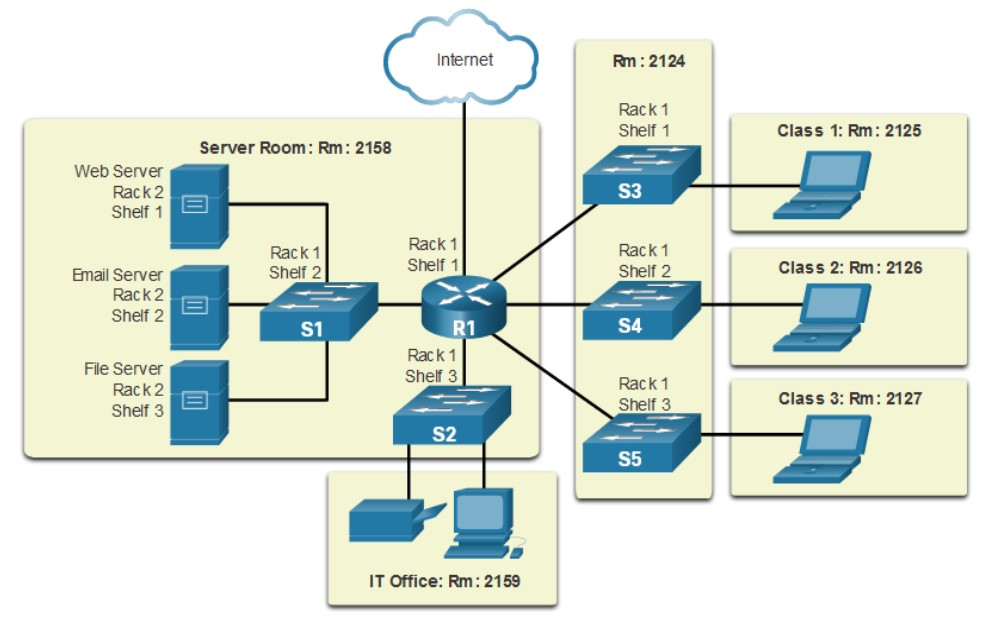
\includegraphics[width=\textwidth]{images/physical_topology_diagram.jpg}
    \caption{Physikalisches Netzwerkdiagramm (\textsuperscript{\textcopyright}Cisco)}
    \end{center}
\end{figure}
\paragraph{Das logische Netzwerkdiagramm}zeigt hingegen über welche \textsl{\textbf{Ports (interfaces)}} die Komponenten angeschlossen sind, sowie welche \textsl{\textbf{Netzwerkadressierung}} gegeben wurde. Merkmale sind Netzwerkadressen, IP-Adressen von Endgeräten, Subnetzmasken, je nach Anwendung auch MAC-Adressen\footnote{Media-Access-Control}. Man spricht auch von einer \textsl{physischen Adresse} oder \textsl{Geräteadresse}.
\begin{figure}[H]
    \begin{center}
    \label{pic:logical_topology}
    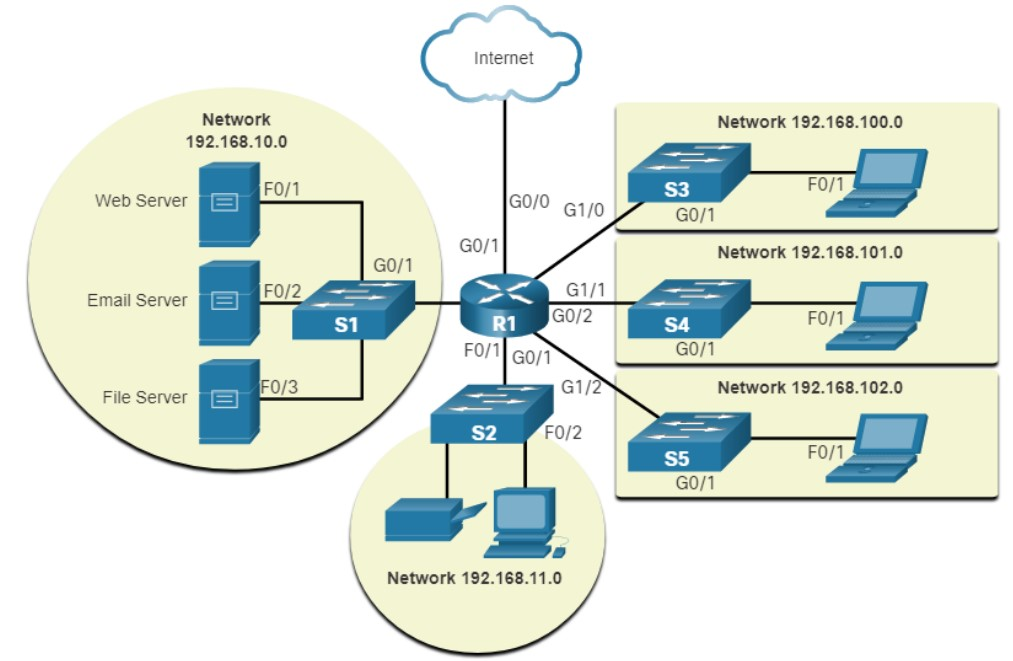
\includegraphics[width=\textwidth]{images/logical_topology_diagram.jpg}
    \caption{Logisches Netzwerkdiagramm (\textsuperscript{\textcopyright}Cisco)}
    \end{center}
\end{figure}
\subsection*{Wie kann man anhand ihrer Grösse Computernetzwerke klassifizieren?}
Es gibt diverse Grössen von Netzwerke. Namentlich sind das:
\begin{itemize}
    \item LAN - Local Area Network. Lokales Netz, mal abgesehen von Subnetzen, auf die Wohnung, Büro oder Firma beschränkt.
    \item MAN - Metropolitan Area Network. Meistens ein Verbund von LANs, welche auf ``kürzere Distanzen'' (bis zu ca. 100 km) durch einen Backbone (Netz mit besonders grosser Übertragungsrate über Glasfaser) vernetzt sind. MANs werden durch Internetdienstanbieter (ISP - Internet Service Provider) betrieben.
    \item WAN - Wide Area Network. Verbund und Backbone von MANs. Salopp: ``Ze Internet''.
\end{itemize}
Die Aufzählung ist nicht abschliessend, denn es gibt z.B. Body Area Network (z.B. medizinische Geräte), Personal Are Network (z.B. Bluetooth), City Area Network, Global Area Network etc.
\subsection*{Wie unterschieden sich LANs und WANs? Was ist ihre Beziehung?}
Sie pflegen eine versteckte Beziehung. Kann ihre Liebe so weiterlodern, inmitten von Intrigen, Verrat und Krieg zwischen den Königshäusern?
\subsection*{Was ist das Internet? Wer besitzt das Internet? Was für Organisationen sind in der Entwicklung des Internets beteiligt?}
Das Internet ist ein globaler Verbund von Rechnernetzwerken, welches die Nutzung von diversen Diensten wie WWW, Email, FTP u.v.m. bietet. Das Internet gehört im Grunde genommen niemandem. Die Organisation IETF\footnote{Internet Engineering Task Force} befasst sich jedoch mit der Weiterentwicklung des Internets, um dessen Funktionsweise zu verbessern.\footnote{\url{https://www.facebook.com/Ballybegpostofficeandgeneralconveniencestore/videos/845703122288697/}}
\subsection*{Was ist der Unterschied zwischen einem Intranet und einem Extranet?}
Auf das Intranet kann nur von innerhalb des LANs zugegriffen werden. Das Extranet bietet hingegen eine Erweiterung des Intranets, die von einer Gruppe von externen Benutzer verwendet werden darf. Extranets bieten Informationen die z.B. an Kunden oder Partnern zugänglich gemacht werden.
\subsection*{Wie verbinden sich normalerweise Häuser, Wohnungen und HomeOffices mit dem Internet?}
Kabelnetz, DSL - Digital Subscriber Line, Dial-Up Modem, GSM - Global System for Mobile Communications, Satellit.
\subsection*{Wie verbinden sich normalerweise Büros und Unternehmern mit dem Internet?}
Dedicated Leased Lines, Metro Ethernet (ethernetbasierte MANs), Business DSL, Satellit.
\subsection*{Was bedeutet Konvergenz im Kontext der Computernetzwerke?}
Voneinander getrennte Netze werden zusammengeführt. Bsp.: klassische Telefonie funktioniert zunehmend über VoIP (Voice over IP).

\begin{figure}[H]
    \begin{center}
    \label{pic:converging_classic}
    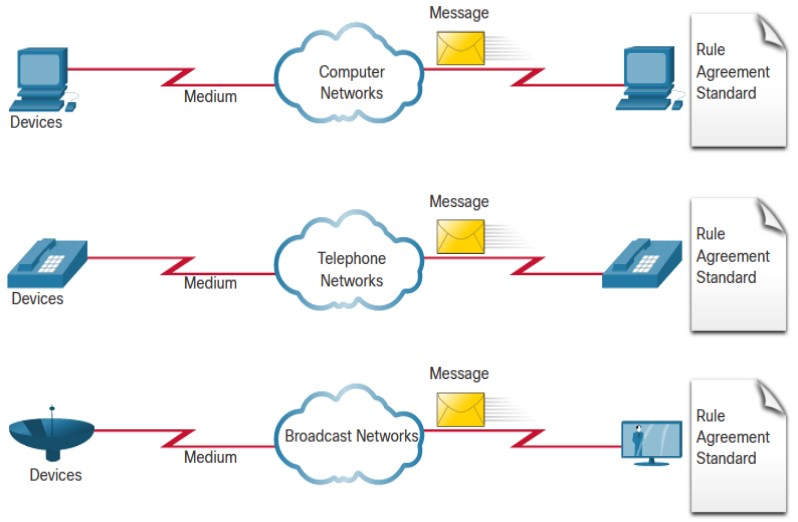
\includegraphics[width=.6\textwidth]{images/converging_network_classic.jpg}
    \caption{Klassisches Netz (\textsuperscript{\textcopyright}Cisco)}
    \end{center}
\end{figure}
\begin{figure}[H]
    \begin{center}
    \label{pic:converging_modern}
    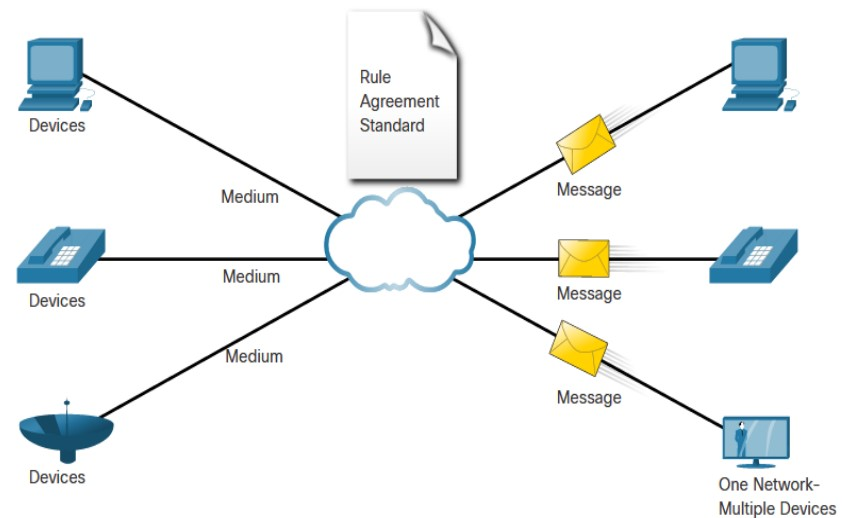
\includegraphics[width=.6\textwidth]{images/converging_network_modern.jpg}
    \caption{Modernes, konvergiertes Netz (\textsuperscript{\textcopyright}Cisco)}
    \end{center}
\end{figure}
\subsection*{Was bedeutet \flqq fault tolerance\frqq{} (Fehlertoleranz) im Kontext der Computernetzwerke? Geben Sie ein Beispiel}
Beim Ausfall einer wichtigen Netzwerkkomponente wie z.B. Router, wird mit redundantem Aufbau eines Netzwerkes die Verbindung weiterhin gewährleistet.
\begin{figure}[H]
    \begin{center}
    \label{pic:fault_tolerance}
    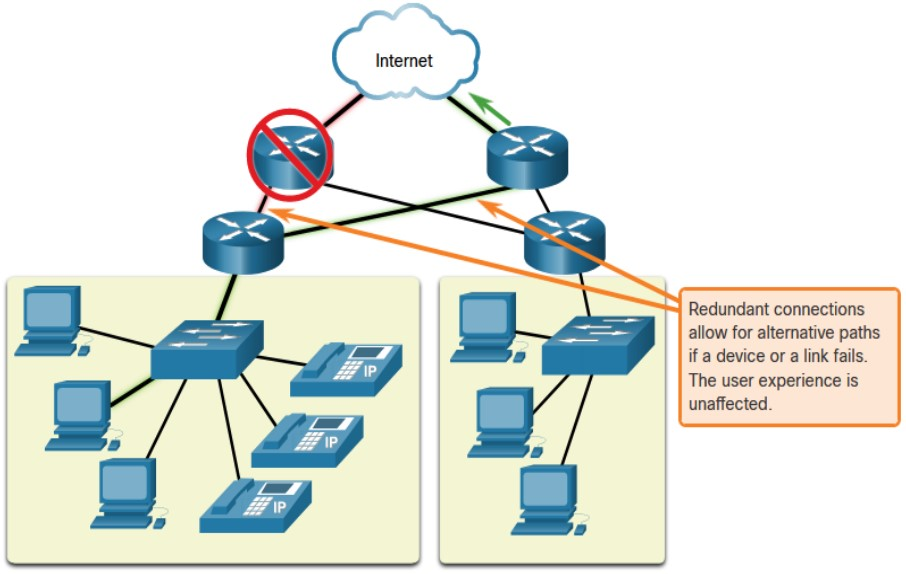
\includegraphics[width=\textwidth]{images/fault_tolerance.jpg}
    \caption{Fault tolerance - Fehlertoleranz (\textsuperscript{\textcopyright}Cisco)}
    \end{center}
\end{figure}
\pagebreak
\subsection*{Was bedeutet \flqq scalability\frqq{} (Skalierbarkeit) im Kontext der Computernetzwerke? Geben Sie ein Beispiel}
Die Skalierbarkeit eines Netzwerkes beschreibt die Fähigkeit/Möglichkeit, ein Netzwerk ohne grossen Aufwand zu erweitern.
\begin{figure}[H]
    \begin{center}
    \label{pic:scalability}
    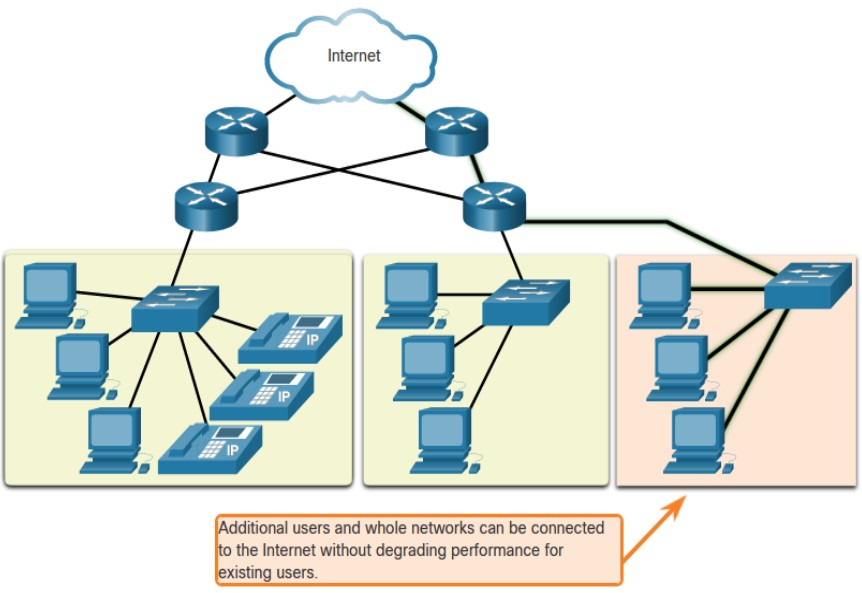
\includegraphics[width=\textwidth]{images/scalability.jpg}
    \caption{scalability - Skalierbarkeit (\textsuperscript{\textcopyright}Cisco)}
    \end{center}
\end{figure}
\subsection*{Was bedeutet \flqq quality of service (QoS)\frqq{} im Kontext der Computernetzwerke? Geben Sie ein Beispiel}
Das QoS dient zur Priorisierung von Netzwerkdiensten und -paketen. Ein Telefonat über VoIP ist wichtiger als eine Webseite, die vielleicht ein paar Millisekunden länger braucht um angezeigt zu werden.
\begin{figure}[H]
    \begin{center}
    \label{pic:qos}
    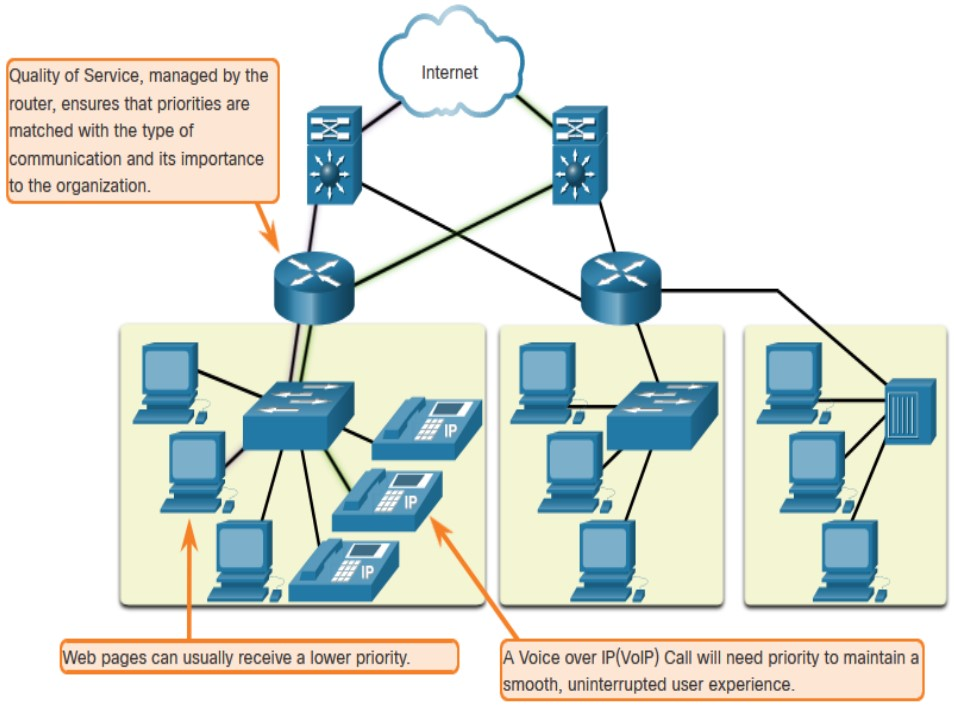
\includegraphics[width=\textwidth]{images/qos.jpg}
    \caption{Quality of service}
    \end{center}
\end{figure}
\subsection*{Wieso ist Netzwerksicherheit wichtig?}
Um Unbefugten nicht versehentlichen oder absichtlichen Zugriff auf das Netzwerk zu gewähren.
\subsection*{Was sind die drei Hauptinformationssicherheitsziele?}
Informationssicherheit ist das höchste Gut, der heilige Grahl der Informatik. Die drei Hauptziele sind:
\begin{itemize}
    \item \textbf{Vertraulichkeit} (confidentiality): lediglich autorisierte Benutzer dürfen entsprechende Daten lesen (z.B. eavesdropper) oder ändern. Dies gilt beim Zugriff auf gespeicherte Daten, wie auch während der Übertragung.
    \item \textbf{Integrität} (integrity): Daten dürfen nicht unbemerkt verändert werden (z.B. man in the middle attack) und alle Änderungen müssen nachvollziehbar sein.
    \item \textbf{Verfügbarkeit} (availability): Verhinderung von Systemausfällen und Gewährleistung der Verfügbarkeit der Daten innerhalb eines definierten Zeitraums.
\end{itemize}
Informationssicherheit wird im Modul ISF - Information Security Fundamentals genauer erarbeitet.
\subsection*{Was ist \flqq BYOD\frqq{} und was sind seine Auswirkungen für Geschäfte und Unternehmen?}
Bring Your Own Device. Für Unternehmen bedeutet dies, dass Komponenten wie Smartphones und Notebooks in das Netzwerk eingebunden werden, welche vielleicht nicht über spezielle Schutzmassnahmen verfügen, als wenn es von der firmeneigenen Informatikabteilung zur Verfügung gestellt werden würde. Umso besser muss das Netzwerk gegen mögliche Bedrohungen, die dieses Philosophie mit sich bringt, geschützt werden.
\subsection*{Was ist \flqq cloud computing\frqq{}? Was für Cloud Arten gibt es?}
Clouds sind verschiedene Dienstleistungen, welche physisch nicht mehr verfügbar sind. Bekanntestes Anwendungsbeispiel ist die File-Cloud. Man hat nicht einen eigenen File-Server, sondern einen externen Anbieter, einen CSP - Could Service Provider, der den Zugang auf die darunterliegende Infrastruktur ermöglicht. Im Grunde gibt es drei Hauptformen von Angeboten:
\begin{itemize}
    \item Software as a Service (SaaS)
    \item Platform as a Service (PaaS)
    \item Infrastructure as a Service (Iaas)
\end{itemize}
Wichtig dabei ist, dass es vier verschiedene Arten von Clouds gibt.
\begin{itemize}
    \item Private
    \begin{itemize}
        \item Ein Unternehmen hat Zugriff auf eine Cloud-Infrastruktur, welche nicht von anderen Firmen genutzt wird (z.B. Dedicated Server). Sicher was Datenschutz angeht, jedoch Verfügbarkeit könnte bei einem Ausfall vielleicht nicht gewährleistet sein.
    \end{itemize}
    \item Public
    \begin{itemize}
        \item Ein Unternehmen teilt sich eine Cloud-Infrastruktur mit anderen Firmen (z.B. Shared Server). Das heisst also, eine Firma bekommt eine definierte Anzahl an Ressourcen zur Verfügung gestellt, hat aber keinen Zugriff auf die gesamte Infrastruktur. Normalerweise sehr hohe Verfügbarkeit, jedoch vom Datenschutz her nicht optimal, da sich Infrastruktur global befindet (Big Brother is watching you), jedoch deswegen auch günstiger im Angebot.
    \end{itemize}
    \item Hybrid
    \begin{itemize}
        \item Hybride Cloud-Infrastrukturen sind in private und public Clouds geteilt. Sensitive Daten werden in der privaten cloud verarbeitet. Operationen die von sensitiven Daten keinen Gebrauch machen können günstig in einer public Cloud verarbeitet werden. Je nach bedarf kann die public Cloud skaliert werden.
    \end{itemize}
    \item Community
    \begin{itemize}
        \item Die Community Cloud ist eine spezielle Form der Cloud. Spezifische Sektoren wie Gesundheits-, Recht-, Finanzbereich u.a. unterliegen oft regulatorischen Konformitäten. Diese ``Sektorsphären'' sind als die Communities anzusehen. CSPs haben aufgrund dieser Konformitäten ein gewisses Angebotsstandard für die Sektoren geschaffen. Vom Datenschutz fast wie eine private Cloud, jedoch von der Funktionalität wie eine public cloud, das heisst, andere Firmen aus derselben Branche nutzen die Cloud mit.
    \end{itemize}
\end{itemize}

Wie bei allem gibt es Vor- und Nachteile bei der Nutzung solcher Angebote.
\subsection*{Was ist die Verbindung zwischen \flqq cloud computing\frqq{} und Computernetzwerken?}
Cloud Computing ist ein Dienstleitungsangebot von Cloud Service Providern. Ein Computernetzwerk ist die darunterliegende Struktur zur Gewährleistung der Datenübertragung.
\newpage
\section*{Formelsammlung}
\subsection*{Einfache lineare Funktionen}
Lineare Funktion
\begin{align*}
    y=&ax+b \\
    y_2-y_1=&a(x_2-x_1)\\
    a=&\frac{y_2-y_1}{x_2-x_1}=\frac{\Delta y}{\Delta x}
\end{align*}

Differenzenquotient
\begin{align*}
    \frac{\Delta y}{\Delta x}=\frac{f(x+\Delta x)-f(x)}{\Delta x}
\end{align*}

\printindex
\end{document}